\section{Session Types}
% Session types are a typing discipline for processes that exchange messages via channels, and implement sessions with structured protocols featuring inputs/outputs, choices, and recursion
As with the applied pi-calculus, session types also have its root in the process calculus, and can be thought of as types for protocols. The idea behind session types, is to describe the communication protocols as a type, that can be checked either at compile-time or runtime, and thus ensure that well-typed programs are well behaved. Essential to session types is the distinction between binary and multiparty communication channels where the binary sessions allow for only two participants, while the multiparty session types can have zero or more participants. Only the basic definitions of session types will be presented here and will refer the reader to articles such as \citeauthor{DBLP:journals/csur/HuttelLVCCDMPRT16} for a deeper introduction. 

\subsection{Binary Session Types}
% maps channels to session types
Session types allow for more structure to channel types, by defining the input, output and linear types. With pi calculus we are only able to keep track of the number of arguments passed through a channel, so preventing that the number of channels send by a participant is different from the recipients expectations. With session type we can define the types passed i.e. \textit{(nat, (nat))} that describes a channel where the recipient expects a pair of values of natural numbers and a channel on which it will reply another natural number. \\ \\
\textbf{Input and Output types} \\
Furthermore it allows for even more refinement, by including information on how channels are used in relation to input and output types. For the input types (processes that can only write on channels) the following notation is used !(\textit{T$_1$,...,T$_n$}). For output types (processes that can only write on channels) the following notation is used ?(\textit{T$_1$,...,T$_n$}). With the previous mentioned channel we can now define it in more detail ?(\textit{nat, }!(\textit{nat})) where the channel can only read a pair of nat values, and write a natural number. \\ \\
\textbf{Linear types} \textit{duality} \\ \\
\textbf{Binary session types} \\ \\


%TODO: Description of session types and what they are used for (behavioural types - which is also behavioural contracts)

\subsection{Multiparty Session Types}
Multiparty session types extend the theory of binary session types to include more than two participants. It does so by describing interactions of a session in a top-down manner as a \textit{global description} of all the messages exchanged, instead of separately looking at the behaviour of each individual channel endpoint, as done so in binary session types. This can ensure protocol conformance and preventing deadlocks, while making it easier to detect errors both manually and by automatic means. As a consequence of multiple participants, \textit{duality} cannot be used directly in multiparty session types due to potential 'invisible' communications determining which future input or output will be willing to receive or send from (TODO: further).  %\autocite{DBLP:journals/csur/HuttelLVCCDMPRT16}.

Taking an example made by \citeauthor{DBLP:journals/csur/HuttelLVCCDMPRT16} of an interaction between three participants of a Client, ATM and the Bank, we can here show how an implementation of global session types look:
\begin{center}
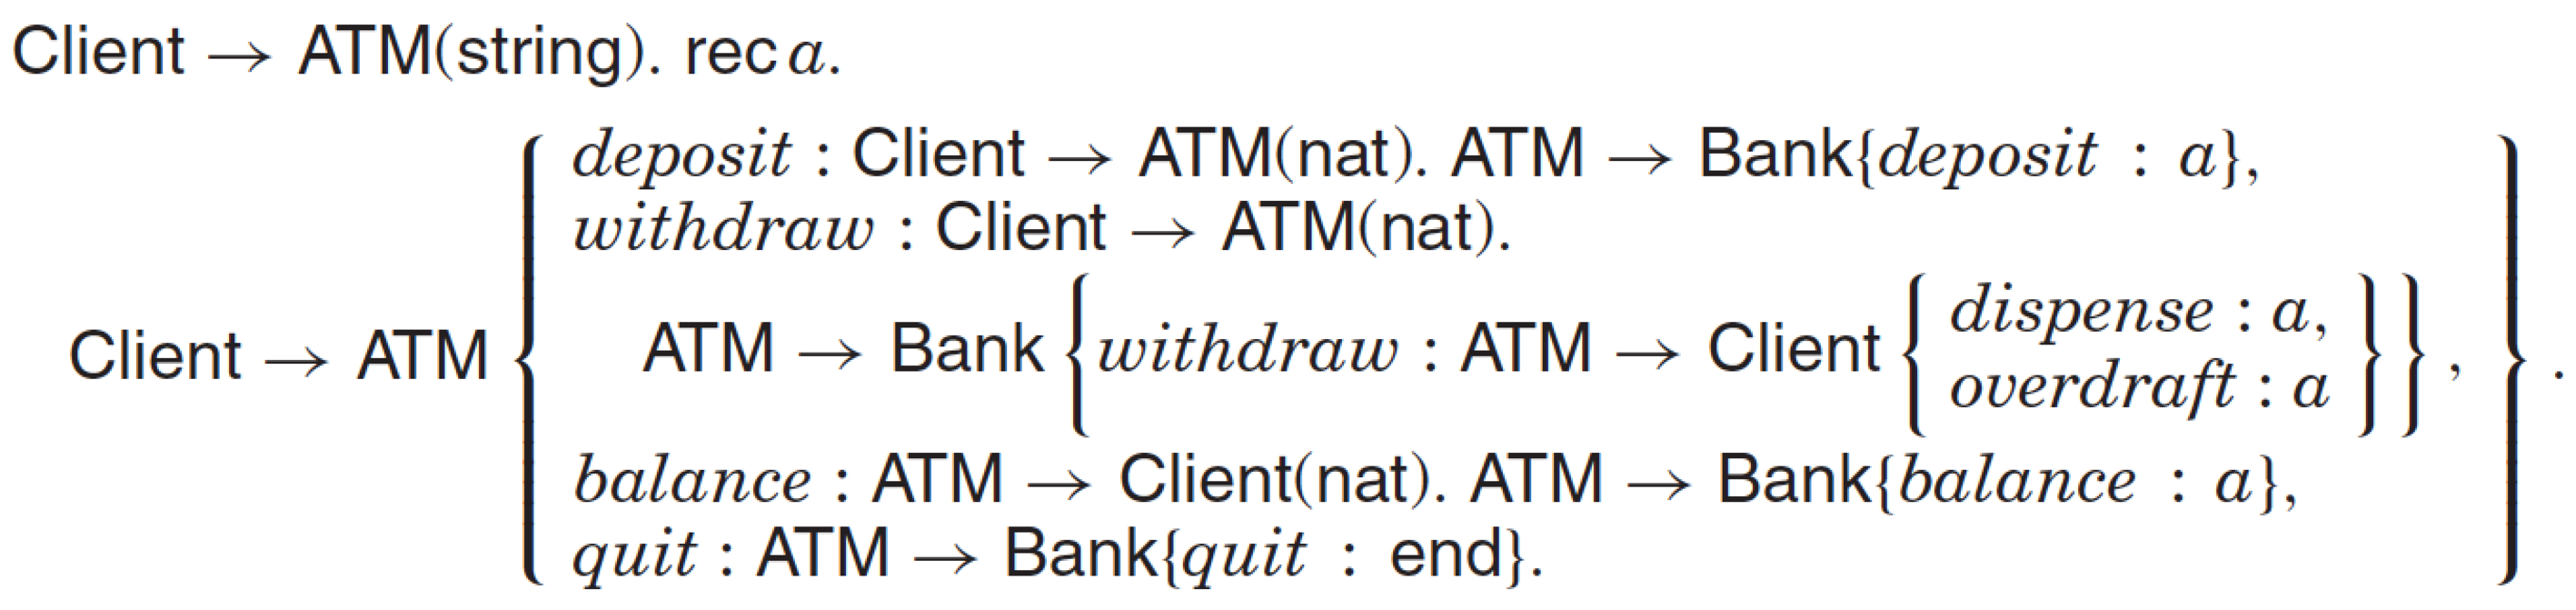
\includegraphics[width=1.0\textwidth, angle=0]{Graphics/Client_ATM.pdf}
\end{center}
First we have that the Client interacts with ATM, where the ATM expects a string input from the Client, and is one of the key interactions operations of \textit{global types}. The ATM then branches and gives the Client four different options to choose from; \textit{deposit, withdraw, balance)} or \textit{quit}, from which the ATM further sends the selected branch to the Bank. Looking at \textit{deposit}, we can tell that the ATM expects a natural number from the client, 
\\ \\
Thus \textit{global types} helps specify the order of the interaction between the three participants in relation to exchanging messages and the order of requests involved.  

\subsection{Research within the field}
TODO: \\ \\

TODO: short description of choreography programming

% note to self: 
% Behavioural Types - describe the dynamic aspects of programs
% Data Types -  describe the fixed structure of data

\iffalse
Maybe Sections instead: \\
 - Behavioural Types \\
 - Session Types \\
 - Examples of global types \\ \\
 \fi